\documentclass[12pt,a4paper]{article}

% --------------------
% Packages
% --------------------
\usepackage[margin=1in]{geometry}
\usepackage{graphicx}
\usepackage{fancyhdr}
\usepackage{setspace}
\usepackage{titlesec}
\usepackage{enumitem}
\usepackage{xcolor}
\usepackage{hyperref}
\usepackage{subcaption}
\usepackage[table]{xcolor}
\usepackage{colortbl}
\usepackage{booktabs}
\usepackage{makecell}
\usepackage{multirow}
\usepackage{svg}
\usepackage{amsmath}

% --------------------
% Paragraph formatting
% --------------------
% \setlength{\parindent}{0pt}  % Remove paragraph indentation
% \setlength{\parskip}{1em}    % Optional: add space between paragraphs

% --------------------
% Project Information
% --------------------
\newcommand{\CompanyName}{Pressure Control Solutions}
\newcommand{\ReportTitle}{Shot Dosing in \\ Pharmaceutical Applications}
\newcommand{\ReportSubTitle}{A Quattroflow QF150 SU Pump with an Equilibar FD \\ in parallel, and with an Equilibar SDO in series}
\newcommand{\AuthorName}{Hubald Verzijl}
\newcommand{\AuthorEmail}{hubald@pressurecontrolsolutions.com}
\newcommand{\VersionNumber}{1.0}
\newcommand{\ReportDate}{March 20, 2026}

\hypersetup{
    colorlinks=true,
    linkcolor=blue,
    filecolor=magenta,      
    urlcolor=cyan,
    pdftitle={\ReportTitle},
    pdfauthor={\AuthorName},
    pdfkeywords={Pressure, Dynamics, Quattroflow, Equilibar, Report},
}

% --------------------
% Header & Footer
% --------------------
\pagestyle{fancy}
\fancyhf{} % Clear default header/footer

% Header
\setlength{\headheight}{30pt}
\fancyhead[L]{%
  
\includegraphics[height=0.75cm]{../images/logo.png}
}
\fancyhead[R]{Report Version \VersionNumber}

% Footer
\fancyfoot[C]{\thepage}

\renewcommand{\headrulewidth}{0.4pt}
\renewcommand{\footrulewidth}{0.4pt}

% --------------------
% Title Page
% --------------------
\begin{document}

\begin{titlepage}
    \thispagestyle{fancy}
    \fancyfoot{} % Clear footer for this page only
    \centering
    \vspace*{2cm}
    {\Huge \bfseries \ReportTitle \par}
    \vspace{0.5cm}
    {\Large \ReportSubTitle \par}
    \vspace{2cm}
    \begin{center}
        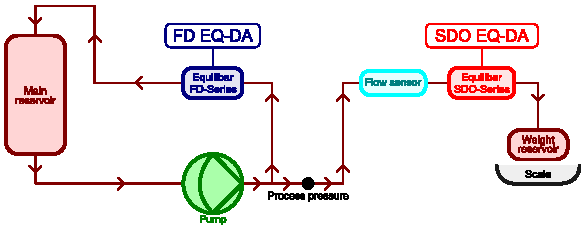
\includegraphics[width=0.8\textwidth]{images/setup.pdf}
    \end{center}
    \vspace{2cm}
    {\Large \CompanyName \par}
    \vspace{0.25cm}
    {\small Author: \AuthorName \par}
    \vspace{0.25cm}
    {\small Report Version: \VersionNumber \par}
    \vspace{0.25cm}
    {\small Date: \ReportDate \par}
    \vfill
\end{titlepage}

\section*{Introduction}
This report presents the results of an experimental evaluation of the shot dosing performance of a Quattroflow QF150 SU pump in combination with an Equilibar SDO backpressure regulator. The experiments were conducted to assess the accuracy and repeatability of the shot dosing process under different pump speeds and control strategies (based on timing and on real-time volume). The report is structured as follows: Section 1 describes the experimental setup, including the components used and their configuration. Section 2 presents the results of open-loop control experiments, while Section 3 discusses the results of closed-loop control experiments. Finally, Section 4 and 5 provides conclusions and recommendations for future investigations.

\tableofcontents
\newpage

\section{Setup}
\subsection{Schematic}
Figure \ref{fig:setup} shows a schematic of the experimental setup used to evaluate the shot dosing performance of the Quattroflow QF150 SU pump in combination with an Equilibar SDO backpressure regulator. The main reservoir is filled with water, which is pumped by the Quattroflow pump. The pump is manually controlled and generates a process pressure that depends on the system resistance. Downstream of the pump, an Equilibar FD-series regulator is installed. The reference pressure on this Equilibar is controlled by the PCS software, ensuring that the process pressure does not exceed the setpoint. In this way, the pump can operate continuously, while the FD-series Equilibar maintains the desired pressure.

A second Equilibar (SDO-series) is also connected downstream of the pump via a coriolis flow sensor. The output of this regulator is collected in a reservoir mounted on a scale. The reference pressure of the SDO Equilibar is controlled by custom software, such that a specific amount of fluid is collected in the reservoir.

\begin{figure}[!ht]
    \centering
    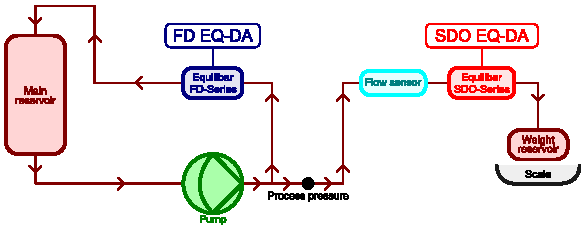
\includegraphics[width=1\textwidth]{images/setup.pdf}
    \caption{Schematic of the experimental setup used to evaluate the shot dosing performance of the Quattroflow QF150 SU pump in combination with an Equilibar SDO backpressure regulator.}
    \label{fig:setup}
\end{figure}

\subsection{Flow sensor}
As a flow sensor, a coriolis SumoFlo 032\footnote{\href{https://www.psgdover.com/biotech/products/coriolis-flow-meters}{https://www.psgdover.com/biotech/products/coriolis-flow-meters}} is used with a maximum flow rate of 3000 ml/min (50 ml/sec). The sensor output is a current signal between 4 and 20 mA, which is converted to a digital signal by the SDO EQ-DA. The flow rate is calculated from the current signal using the following formula:
\begin{equation}
    Q = \frac{I - 4}{16} \cdot 3000,
\end{equation}
where $Q$ is the flow rate in ml/min and $I$ is the current signal in mA. To maximize the bandwidth of the sensor, any onboard filtering (by the SumoFlo) is disabled.

\newpage
\section{Open-loop control}
\subsection{Method}
For the open-loop control experiments, the Quattroflow pump is operated at fixed speeds of 250, 500, 750, and 1000 rpm. Since the pump uses a membrane design, the corresponding flow rates are expected to be 300, 600, 900, and 1200 mL/min, respectively.  

During all experiments, the FD-series Equilibar regulator is set to a reference pressure of 1.5 bar, limiting the process pressure to this value while the pump is operating continuously. The SDO-series Equilibar is initially set to a reference pressure of 2 bar, which keeps it fully closed. At each pump speed, the SDO reference pressure is allowed to stabilize at 2 bar for 10 seconds before a setpoint of 0 bar is applied for 5 seconds. The process pressure is then increased back to 2 bar. This sequence is referred to as a shot. Four shots are performed at each pump speed. After each shot, the scale reading is recorded and tared to zero before the next shot. During the experiments, data is recorded at a frequency of 1000 Hz, including the reference pressure, the reference setpoint, temperature, valve positions, and flow.

\subsection{Results}
\subsubsection{Measurement graphs}
Figure \ref{fig:open_loop_results} shows the results of the open-loop control experiments at a pump speed of 250 rpm. The four shots look fairly similar. The first shot is shown in more detail in figure \ref{fig:shot_1} and all shots at different pump speeds in Figure \ref{fig:all_shots}. The process pressure (orange) follows the reference pressure (gray) closely, with some fluctuations around the setpoint. The valve positions show that both the inlet and outlet valves are fully open during the shot, allowing for maximum flow. The flow rate (third graph) shows a clear increase during the shot, reaching flows around 300 ml/min, which is consistent with the expected flow rate for this pump speed.

\begin{figure}[!ht]
    \centering
    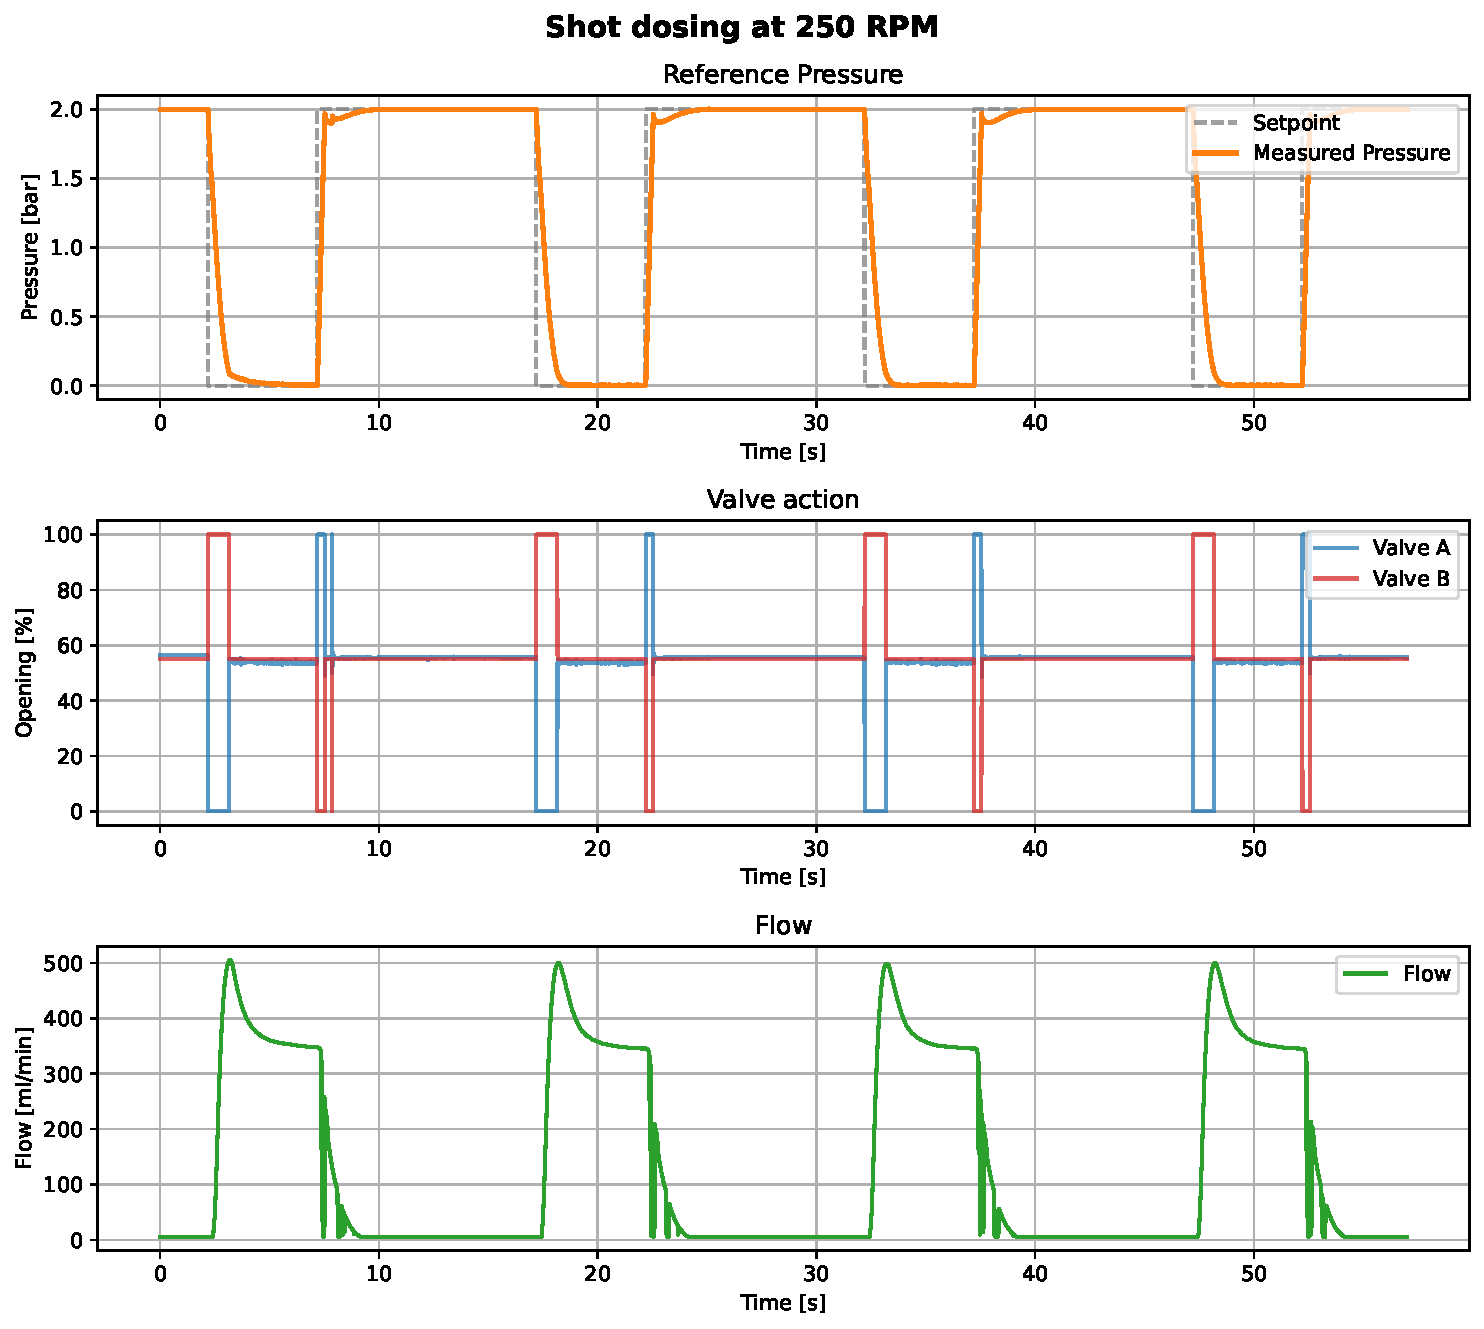
\includegraphics[width=1\textwidth]{images/open_loop_flow_overview_250RPM.pdf}
    \caption{Results of the open-loop control experiments at a pump speed of 250 rpm. The top graph shows the setpoint of the reference pressure on the FD-series Equilibar (gray) and the measured process pressure (orange). The second graph shows the valve positions to create these reference pressures. The in- and outlet valves are fully open to reach the setpoint as fast as possible. The output of the SumoFlo (transformed to ml/min) is shown in the third graph. Four shots are visible.}
    \label{fig:open_loop_results}
\end{figure}

\begin{figure}[!ht]
    \centering
    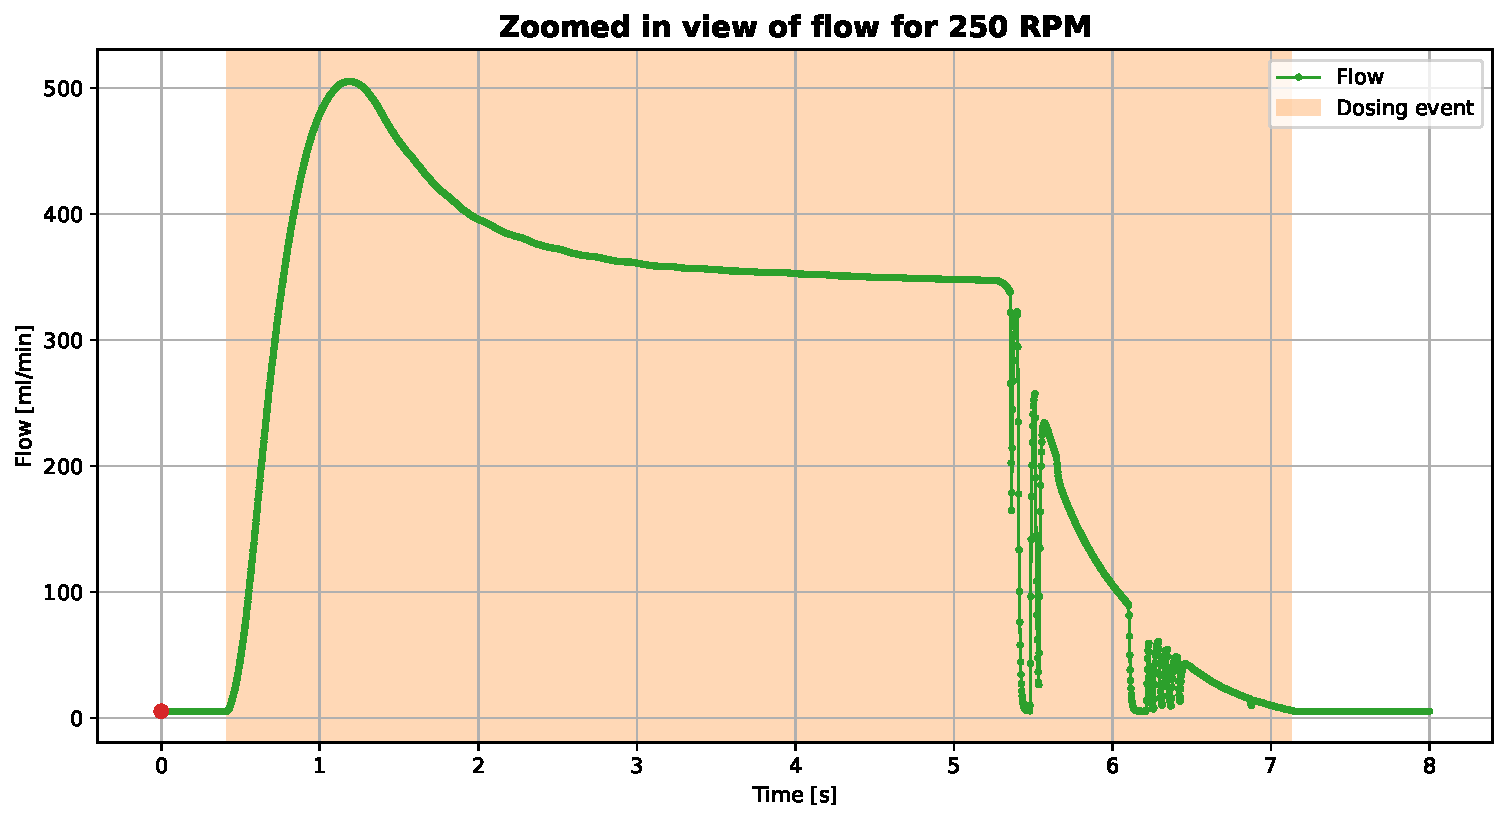
\includegraphics[width=1\textwidth]{images/open_loop_flow_zoomed_250RPM.pdf}
    \caption{Detailed view of the first shot at a pump speed of 250 rpm. The small green dots represent a single measurement point. The sensor gives a positive output flow rate when there is no flow, which is represented by the red dot: it is slightly above 0. The orange area is defined as a dosing event (defined as a flow of $>$ 6 ml/min), which is later used to calculate the amount of fluid dosed during the shot.}
    \label{fig:shot_1}
\end{figure}

\begin{figure}
    \centering
    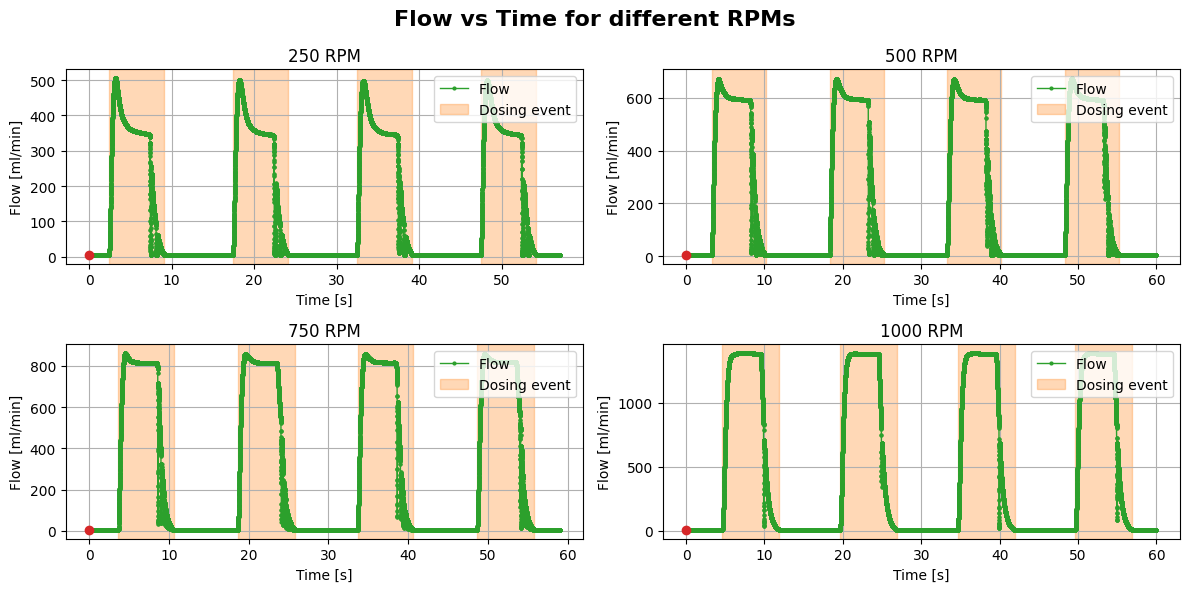
\includegraphics[width=1\textwidth]{images/open_loop_flow_all_cases.png}
    \caption{Results of the open-loop shot dosing control experiments at pump speeds of 250, 500, 750, and 1000 rpm with the Equilibar SDO activated four consecutive times.}
    \label{fig:all_shots}
\end{figure}

\clearpage
\subsubsection{Dose volumes}
For every shot, the amount of fluid dosed is calculated by integrating the flow rate over the duration of the shot (the orange area in figure \ref{fig:shot_1}) using: 
\begin{equation}
    V = \sum_{t=t_1}^{t_2} \left[Q(t) - Q(0)\right] \cdot \Delta t,
    \label{eq:sum}
\end{equation}
where $V$ is the volume of fluid dosed in ml, $Q(t)$ is the flow rate at time $t$ in ml/s, $Q(0)$ is the initial flow rate (red dots in Figures \ref{fig:shot_1} and \ref{fig:all_shots}), and $t_1$ and $t_2$ are the start and end times of the shot. The raw measurements, including the standard deviation (SD), are shown in Table \ref{tab:shot_results}.

\begin{table}[!ht]
\centering
\begin{tabular}{c cc cc cc cc cc}
\toprule
\multirow{2}{*}{\makecell{\textbf{Pump} \\ \textbf{Speed} \\ (RPM)}}
& \multicolumn{2}{c}{\textbf{Shot 1}}
& \multicolumn{2}{c}{\textbf{Shot 2}}
& \multicolumn{2}{c}{\textbf{Shot 3}}
& \multicolumn{2}{c}{\textbf{Shot 4}}
& \multicolumn{2}{c}{\textbf{SD}} \\
\cmidrule(lr){2-3} \cmidrule(lr){4-5} \cmidrule(lr){6-7} \cmidrule(lr){8-9} \cmidrule(lr){10-11}
& \makecell{\textbf{$V_{\text{SF}}$} \\ (ml)} & \makecell{\textbf{$V_{\text{Scale}}$} \\ (g)}
& \makecell{\textbf{$V_{\text{SF}}$} \\ (ml)} & \makecell{\textbf{$V_{\text{Scale}}$} \\ (g)}
& \makecell{\textbf{$V_{\text{SF}}$} \\ (ml)} & \makecell{\textbf{$V_{\text{Scale}}$} \\ (g)}
& \makecell{\textbf{$V_{\text{SF}}$} \\ (ml)} & \makecell{\textbf{$V_{\text{Scale}}$} \\ (g)}
& \makecell{\textbf{$V_{\text{SF}}$} \\ (ml)} & \makecell{\textbf{$V_{\text{Scale}}$} \\ (g)} \\
\midrule
250 & 31.75 & 30 & 31.37 & 30 & 31.46 & 30 & 31.33 & 30 & 0.17 & 0.00 \\
500 & 50.59 & 48 & 50.68 & 48 & 50.26 & 48 & 51.02 & 47 & 0.27 & 0.43 \\
750 & 68.74 & 64 & 70.66 & 64 & 68.17 & 64 & 70.89 & 64 & 1.18 & 0.00 \\
1000 & 115.55 & 105 & 115.75 & 108 & 115.22 & 105 & 115.46 & 106 & 0.19 & 1.22\\
\bottomrule
\end{tabular}
\caption{Dosed volumes obtained via SumoFlo integration ($V_{\text{SF}}$) and scale measurements ($V_{\text{Scale}}$) for different pump speeds.}
\label{tab:shot_results}
\end{table}

The interpreted values allow calculation of the percentage error of the sensor fusion (SF) volume relative to the scale measurements:
\begin{equation}
    \text{Percentage Error} = \left| \frac{V_{\text{SF}} - V_{\text{Scale}}}{V_{\text{Scale}}} \right| \cdot 100\%,
\end{equation}
where $V_{\text{SF}}$ is the volume calculated from the SumoFlo sensor fusion and $V_{\text{Scale}}$ is the volume measured by the scale. These results are shown in Table \ref{tab:percentage_error}. The color coding in the table indicates the magnitude of the percentage error: green for 0–5\%, yellow for 5–10\%, and orange for above 10\%. From the results, it is clear that higher pump speeds lead to higher percentage errors.

\begin{table}[!ht]
\centering
\begin{tabular}{c cccc}
\toprule
\makecell{\textbf{Pump Speed} (RPM)}
& \textbf{Shot 1 (\%)}
& \textbf{Shot 2 (\%)}
& \textbf{Shot 3 (\%)}
& \textbf{Shot 4 (\%)} \\
\midrule
250 & \cellcolor{yellow!25}5.84 & \cellcolor{green!15}4.56 & \cellcolor{green!15}4.85 & \cellcolor{green!15}4.42 \\
500 & \cellcolor{yellow!25}5.39 & \cellcolor{yellow!25}5.58 & \cellcolor{green!15}4.70 & \cellcolor{yellow!25}8.56 \\
750 & \cellcolor{yellow!25}7.41 & \cellcolor{orange!30}10.40 & \cellcolor{yellow!25}6.52 & \cellcolor{orange!30}10.77 \\
1000 & \cellcolor{orange!30}10.05 & \cellcolor{yellow!25}7.18 & \cellcolor{yellow!25}9.73 & \cellcolor{yellow!25}8.93 \\
\bottomrule
\end{tabular}
\caption{Percentage error of the SumoFlo integration volume ($V_{\text{SF}}$) relative to scale measurements ($V_{\text{Scale}}$) for different pump speeds. Color indicates error magnitude.}
\label{tab:percentage_error}
\end{table}

\clearpage
\section{(Semi-)Closed-loop control}
Based on the results of the open-loop control experiments, a closed-loop control experiment is set up to evaluate whether the performance of the shot dosing can be improved by controlling the reference pressure of the SDO-series Equilibar in real-time based on the flow measurements from the SumoFlo sensor.

\subsection{Method}
The same setup is used, but now the reference pressure of the SDO-series Equilibar is controlled by custom software to achieve a specific target volume. The SumoFlo sensor integration is performed in real-time, and the reference pressure of the SDO-series Equilibar is set to 2 bar when the target volume is reached, which closes the valve and stops the flow. Again, four shots are performed at each pump speed of 250, 500, 750, and 1000 rpm. The target volumes are set to 50 ml.

\subsection{Results}

\subsubsection{Measurement graphs}
The raw measurement graphs look very similar to the open-loop control experiments, but now the reference pressure of the SDO-series Equilibar is increased to 2 bar at the moment the target volume is reached. As this happens within fractions of a second, the difference is hard to see in the graphs. 

\subsubsection{Dose volumes}
More interesting is to look at the dose volumes. The results are shown in Table \ref{tab:closed_loop_results}. The percentage error of the sensor fusion volume relative to the scale measurements is calculated and shown in Table \ref{tab:closed_loop_percentage_error}. Compared to the open-loop control experiments, the percentage errors are significantly reduced, especially at higher pump speeds.

\begin{table}[!ht]
\centering
\begin{tabular}{c cc cc cc cc cc}
\toprule
\multirow{2}{*}{\makecell{\textbf{Pump} \\ \textbf{Speed} \\ (RPM)}}
& \multicolumn{2}{c}{\textbf{Shot 1}}
& \multicolumn{2}{c}{\textbf{Shot 2}}
& \multicolumn{2}{c}{\textbf{Shot 3}}
& \multicolumn{2}{c}{\textbf{Shot 4}}
& \multicolumn{2}{c}{\textbf{SD}} \\
\cmidrule(lr){2-3} \cmidrule(lr){4-5} \cmidrule(lr){6-7} \cmidrule(lr){8-9} \cmidrule(lr){10-11}
& \makecell{\textbf{$V_{\text{SF}}$} \\ (ml)} & \makecell{\textbf{$V_{\text{Scale}}$} \\ (g)}
& \makecell{\textbf{$V_{\text{SF}}$} \\ (ml)} & \makecell{\textbf{$V_{\text{Scale}}$} \\ (g)}
& \makecell{\textbf{$V_{\text{SF}}$} \\ (ml)} & \makecell{\textbf{$V_{\text{Scale}}$} \\ (g)}
& \makecell{\textbf{$V_{\text{SF}}$} \\ (ml)} & \makecell{\textbf{$V_{\text{Scale}}$} \\ (g)}
& \makecell{\textbf{$V_{\text{SF}}$} \\ (ml)} & \makecell{\textbf{$V_{\text{Scale}}$} \\ (g)} \\
\midrule
250 & 51.59 & 50 & 51.47 & 50 & 51.49 & 50 & 51.41 & 50 & 0.07 & 0.43 \\
500 & 54.90 & 52 & 55.23 & 52 & 55.19 & 52 & 55.73 & 52 & 0.30 & 0.00 \\
750 & 58.41 & 55 & 58.18 & 55 & 57.64 & 55 & 60.06 & 56 & 0.90 & 0.50 \\
1000 & 59.97 & 55 & 59.85 & 55 & 60.06 & 55 & 59.84 & 55 & 0.09 & 0.50 \\
\bottomrule
\end{tabular}
\caption{Dosed volumes obtained via SumoFlo integration ($V_{\text{SF}}$) and scale measurements ($V_{\text{Scale}}$) for different pump speeds.}
\label{tab:closed_loop_results}
\end{table}

\begin{table}[!ht]
\centering
\begin{tabular}{c cccc}
\toprule
\makecell{\textbf{Pump Speed} (RPM)}
& \textbf{Shot 1 (\%)}
& \textbf{Shot 2 (\%)}
& \textbf{Shot 3 (\%)}
& \textbf{Shot 4 (\%)} \\
\midrule
250 & \cellcolor{green!15}3.19 & \cellcolor{green!15}2.93 & \cellcolor{green!15}2.98 & \cellcolor{green!15}0.81 \\
500 & \cellcolor{yellow!25}5.58 & \cellcolor{yellow!25}6.20 & \cellcolor{yellow!25}6.13 & \cellcolor{yellow!25}7.17 \\
750 & \cellcolor{yellow!25}8.17 & \cellcolor{yellow!25}5.79 & \cellcolor{yellow!25}6.74 & \cellcolor{yellow!25}9.20 \\
1000 & \cellcolor{yellow!25}9.04 & \cellcolor{yellow!25}6.88 & \cellcolor{yellow!25}9.19 & \cellcolor{yellow!25}6.85 \\
\bottomrule
\end{tabular}
\caption{Percentage error of the SumoFlo integration volume ($V_{\text{SF}}$) relative to scale measurements ($V_{\text{Scale}}$) for different pump speeds. Color indicates error magnitude.}
\label{tab:closed_loop_percentage_error}
\end{table}

\newpage
\section{Conclusion}
\begin{itemize}
    \item The open-loop control experiments showed that the shot dosing performance of the Quattroflow QF150 SU pump in combination with an Equilibar SDO backpressure regulator is reasonably accurate at lower pump speeds, but percentage error increases at higher pump speeds. This holds for both open-loop and closed-loop cases.
    \item The (semi-)closed-loop strategy, where the reference pressure of the SDO-series Equilibar is adjusted in real-time based on flow measurements, creates the opportunity to give a specific target volume and to stop the flow immediately when this target is reached. However, with the current algorithm, deviations of almost 10\% are observed at higher pump speeds.
    \item The shot dosing volume is consistently larger than the measured volume on the scale. Additionally, the percentage error increases with pump speed. The first observation may be due to the SumoFlo sensor not being properly calibrated, while the second may be caused by the SDO-series Equilibar closing too slowly, creating an overshoot in the dosed volume, especially at higher pump speeds.
    \item The closing behavior of the SDO-series Equilibar causes fast fluctuations in the flow rate, which may lead to inaccurate volume measurements by the SumoFlo sensor and could cause deviations in the integration to calculate the dosed volume.
\end{itemize}

\clearpage
\section{Recommendations for future investigation}
\begin{itemize}
    \item Add a chapter 4 about 'real closed-loop control' and investigate how to close the SDO-series Equilibar to avoid overshoot in the dosed volume. The semi-closed-loop approach does not work sufficiently well. Two options could be implemented:
    \begin{itemize}
        \item Gradually decrease the flow by adjusting the reference pressure of the SDO-series Equilibar before the target dosing volume is reached, instead of abruptly changing to 2 bar. This could be implemented using a PID controller.
        \item Keep the on-off control strategy, but use an algorithm to predict when the target volume will be reached and close the SDO-series Equilibar slightly before this moment.
    \end{itemize}
    \item Include a scale that measures the dose volume with digits after the decimal point, which allows for a more accurate measurement of the dosed volume and thus a more accurate calculation of the percentage error.
    \item Calibrate the SumoFlo sensor to ensure that the flow measurements are accurate and that the sensor gives a zero output when there is no flow.
    \item Investigate if the integration of a pulsed flow through the SumoFlo sensor is correct and whether the fluctuations in the flow rate caused by the SDO-series Equilibar closing are affecting the accuracy of the volume calculations.
\end{itemize}

\newpage
\section*{Version control}
\addcontentsline{toc}{section}{Version control}

\begin{tabular}{|c|c|c|}
\hline
Version & Date & Description \\
\hline
1.0 & March 20, 2026 & Initial draft \\
\hline
\end{tabular}

\end{document}